\section{Mirror}


\begin{figure*}[t]
    \centering
    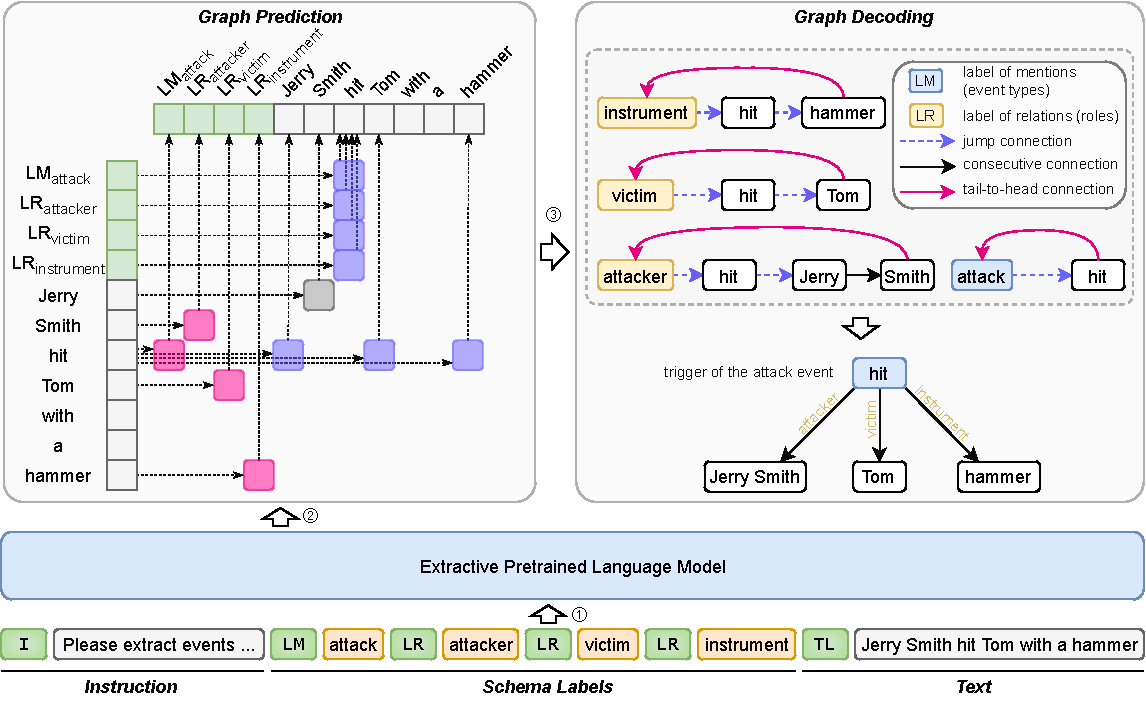
\includegraphics[width=\textwidth]{figs/Model Framework.pdf}
    \caption{Model framework (best viewed in color).}
    \label{fig:model-framework}
\end{figure*}

In this section, we introduce the Mirror framework.
We first address the unified data input format to the model, then introduce the unified task formulation and the model structure.

\subsection{Unified Data Interface}

To make the model able to handle different IE tasks, we propose a unified data interface for the model input.
As shown in Figure~\ref{fig:unified-data-interface}, there are three parts: the \textit{instruction}, the \textit{schema labels}, and the \textit{text}.
The instruction is composed of a leading token \verb|[I]| and a natural language sentence.
The leading token indicates the instruction part while the sentence tells the model what it should do.
For example, the instruction of NER could be \textit{Please identify any possible entities in the given text and label them with the following types}.
The instruction is the question in Machine Reading Comprehension (MRC) and Question Answering (QA) datasets.

The schema labels are task ontologies that used for schema-guided extraction.
This part is consists of special token labels (\verb|[LM]|, \verb|[LR]| and \verb|LC|) and corresponding label texts.
Among the special tokens, \verb|[LM]| denotes the label of mentions (or event types), \verb|[LR]| denotes the label of relations (or argument roles), and \verb|[LC]| denotes the label of classes.
\verb|[LC]| token is designed for classification tasks when pretraining.

The text part is the input text that the model should extract information from.
It is composed of a leading token (\verb|[TL]| or \verb|[TP]|) and a natural language sentence.
If the leading token is \verb|[TL]|, the model should link labels from schema labels to spans in the text.
While the \verb|[TP]| token indicates the target spans are only in the text, and the model should extract information from the text without schema labels.
The \verb|[TP]| label is used in the pretraining stage to make the model able to extract information in MRC tasks without schema.
In classification tasks when pretraining, the model should not extract anything from the text part.
So we add a special background area with a leading token \verb|[B]| to distinguish from extractive texts.

With the above three parts, we can formulate classification, extractive MRC (and extractive QA), multi-choice MRC, and IE tasks into a unified data interface, and the model can be trained in a unified way even the model is not based on generative language models.
For the robust model training, we manually collect 57 datasets across 5 tasks to make a corpus for model pretraining.
To balance the number of examples in each task, we randomly sample instances for each dataset.
If the number of instances in a dataset is less than the sampling value, we keep the original dataset unchanged and do not perform over sampling.
For NER, RE and EE tasks, we manually design a set of instructions, and randomly pick one of them for each sample.
The number of instructions for each IE task is listed in Table~\ref{tab:pretrain-dataset-statistics}.
For more detailed statistics on each dataset, please refer to Appendix~\ref{sec:appendix_data}.

\begin{table}[t]
    \centering
    \resizebox{\columnwidth}{!}{
    \begin{tabular}{lrrrr}
        \toprule
        Task & \#Dataset & \#Samples/Dataset & \#Instruction & \#Instance \\
        \midrule
        NER & 15 & 20,000 & 42 & 171,609 \\
        Cls$^{\clubsuit}$ & 27 & 5,000 & 54,070 & 134,758 \\
        RE & 9 & 20,000 & 9 & 123,876 \\
        MRC$^{\heartsuit}$ & 5 & 30,000 & 75,200 & 85,658 \\
        EE & 1 & All & 40 & 2,898 \\
        \midrule
        Total & 57 & - & - & 518,799 \\
        \bottomrule
    \end{tabular}
    }
    \caption{
        Pretraining dataset statistics.
        $^{\clubsuit}$ Classification tasks contain multi-choice MRC datasets.
        $^{\heartsuit}$ MRC stands for both extractive QA and extractive MRC datasets.
    }
    \label{tab:pretrain-dataset-statistics}
\end{table}

\subsection{Multi-slot Tuple and Multi-span Cyclic Graph}

We formulate IE tasks as a unified multi-slot tuple extraction problem.
As exemplified in Figure~\ref{fig:unified-data-interface}, in the RE task, the model is expected to extract a 3-slot tuple like \texttt{(relation, head entity, tail entity)}.
Here, the tuple is \texttt{(LR$_{\text{friend of}}$, Jerry Smith, Tom)}.
The length of tuple slots could vary across tasks, so Mirror is capable of n-ary extraction problems.

As shown in Figure~\ref{fig:multi-span-cyclic-graph} and the top right of Figure~\ref{fig:model-framework}, we formulate multi-slot tuples into a unified multi-span cyclic graph, and regard labels as the leading tokens in schema labels.
There are three types of connections in the graph: the \textbf{\textit{consecutive}} connection, the \textbf{\color[HTML]{695efb} \textit{jump}} connection, and the \textbf{\color[HTML]{E9087F}\textit{tail-to-head}} connection.
The \textbf{\textit{consecutive}} connection is adopted to \textbf{spans in the same entity}.
For an entity that has multiple tokens, the consecutive connection connects from the first token to the last token.
As shown in Figure~\ref{fig:model-framework}, ``Jerry'' connects to ``Smith''.
If there is only one token in an entity, the consecutive connection is not used.
For example, entities in ``muscle pain and fatigue'' contains two entities ``muscle pain'' and ``muscle fatigue''.
The consecutive connection is used to connect from ``muscle'' to ``pain'', and ``muscle'' to ``fatigue''.
The \textbf{\color[HTML]{695efb} \textit{jump}} connection connects \textbf{different slots} in a tuple.
Schema labels and spans from texts are in different slots, so they are connected in jump connections.
In addition, the head entity and the tail entity of a relation triplet are in different slots, so they are also connected in jump connections.
The \textbf{\color[HTML]{E9087F}\textit{tail-to-head}} connection helps \textbf{locate the start \& end boundaries}, and forms a cycle in the graph.
It connects from the last token of the last slot to the first token of the first slot in a tuple.

In practice, we convert the answer of each slot into span positions.
For schema labels, we use the position of leading tags instead of label texts.
For text spans like entities, the position is a one-digit number if there is only one character, otherwise the start and end positions are listed.
For example, the 3-slot relation tuple \texttt{(LR$_{\text{friend of}}$, Jerry Smith, Tom)} will be converted into (9 {\color[HTML]{695efb} $\vdots$} 16 $\to$ 17 {\color[HTML]{695efb} $\vdots$} 22), where $\vdots$ denotes the jump connection, $\to$ stands for the consecutive connection, 9 is the position of \texttt{LR$_{\text{friend of}}$}, 16 and 17 express \textit{Jerry Smith}, and 22 is the position of \textit{Tom}.
There is also a tail-to-head connection from 22 to 9.
The corresponding graph decoding algorithm is shown in Algorithm~\ref{alg:mcg-decoding}.
During inference, we first find the forward chain (9,16,17,22), and then verify the chain with tail-to-head connection (22$\to$9).
After that, the multi-slot tuple is revealed with jump connections(9$\vdots$16) and (17$\vdots$22).

\begin{algorithm}[t]
    \renewcommand{\algorithmicrequire}{\textbf{Input:}}
    \renewcommand{\algorithmicensure}{\textbf{Output:}}
    \caption{\textsc{Multi-span Cyclic Graph Decoding}}
    \label{alg:mcg-decoding}
    \begin{algorithmic}[1]
        \Require Adjacency matrix $\mathcal{A}$
        \Ensure A set of multi-slot tuples $\mathcal{T}$
        \State $\mathcal{T} \gets \{\}$
        \State $\tilde{\mathcal{A}} \gets \mathcal{A}^{c} | \mathcal{A}^{j}$ \Comment{merge consecutive and jump connections}
        \State Find forward chains $\mathcal{C}$ from $\tilde{\mathcal{A}}$
        \For {$c \in \mathcal{C}$}
            \Comment{find legal paths with tail-to-head connections}
            \If{$c$ meets the need in $\mathcal{A}^{t}$}
                \State split $c$ into a tuple $t$ via $\mathcal{A}^j$
                \State $\mathcal{T} \gets \mathcal{T} \cup t$
            \EndIf
        \EndFor
        \State \Return $\mathcal{T}$
    \end{algorithmic}
\end{algorithm}


\subsection{Model Structure}

With the unified data interface and the multi-span cyclic graph, we propose a unified model structure for IE tasks.
For each token $x_i$ from the inputs, Mirror transforms it into a vector $h_i \in \mathbb{R}^{d_h}$ via a BERT-style extractive pretrained language model (PLM).
Similar to \citet{ner-as-dp}, we use biaffine attention to obtain the adjacency matrix $\mathcal{A}$ of the multi-span cyclic graph.
Mirror calculates the linking probability $p_{ij}^{k}, k \in \{\text{consecutive}, \text{jump}, \text{tail-to-head}\}$ between $x_i$ and $x_j$.
The final $\mathcal{A}$ is obtained via thresholding.
\begin{equation}
    \label{eqn:sim_calc}
    \begin{gathered}
    \tilde{h_i} = \text{FFNN}_{s}\left(h_i\right), \quad \tilde{h_j} = \text{FFNN}_{e}\left(h_j\right) \\
    p_{ij}^{k} = \text{sigmoid}\left(\tilde{h_i}^{\top} U \tilde{h_j} / \sqrt{d_h}\right)
    \end{gathered} \\
\end{equation}
\begin{equation}
    \label{eqn:adjacent}
    \mathcal{A}_{i,j}^{k} = \begin{cases}
        1 & p_{ij} > \gamma \\
        0 & \text{otherwise}
    \end{cases}
\end{equation}
where $U \in \mathbb{R}^{d_h \times 3 \times d_h}$ is trainable parameter, and 3 denotes consecutive, jump and tail-to-head connections.
$\text{FFNN}$ is the feed forward neural network with rotary positional embedding as introduced in \citet{roformer}.
The FFNN is composed of linear transformation, GELU activation function~\cite{gelu} and dropout~\cite{dropout}.

During training, we adopt the imbalance-class multi-label categorical cross entropy~\cite{global_pointer} as the loss function.

\begin{equation}
    \label{eqn:loss}
    \mathcal{L}(i,j) = \log \left(1 + \sum_{\Omega_{\text{neg}}} e^{p_{ij}^{k}}\right) + \log \left(1 + \sum_{\Omega_{\text{pos}}} e^{-p_{ij}^{k}}\right)
\end{equation}
where $\Omega_{\text{neg}}$ stands for negative samples ($\mathcal{A}_{ij}^{k}=0$), and $\Omega_{\text{pos}}$ denotes positive samples ($\mathcal{A}_{ij}^{k}=1$).
